\documentclass{../../template/tp}
\usepackage[utf8]{inputenc}
\usepackage{ucs}
\usepackage[frenchb]{babel}
\usepackage[T1]{fontenc}

\usepackage{graphicx}
\graphicspath{{figures/}}
\usepackage{amssymb}
\usepackage{amsmath}
\usepackage{wasysym} %smiley
\usepackage{hyperref}% hyperliens
\usepackage{tikz}
\usetikzlibrary{babel,positioning,calc}
\usepackage[]{circuitikz}
\usepackage{textcomp}
% \usepackage{minted}
\usepackage[long]{datetime}
\usepackage{gensymb} % \ohm, celsius
\usepackage{framed}
\usepackage{pdfpages}
\usepackage{mathastext} % math as standfard text : units are respecting typography conventions.
\usepackage{xspace} % typographie IN
\usepackage[all]{hypcap} %lien pointe en haut des figures
\langexam{frenchb}
\usepackage{fancyhdr}

\newboolean{koriG}
\ifx\koriG\undefined
\correction{false}
\else
\correction{true}
\fi


% \correction{true}

\author{GEI}


\newcommand{\itgv}[1]{\ifthenelse{\boolean{corrige}}{{\color{blue}#1}}{}} %si corrigé vrai...
\newcommand{\ifgv}[1]{\ifthenelse{\boolean{corrige}}{}{#1}} %si corrigé vrai...
%% fancy header & foot
\pagestyle{fancy}
\lhead{[EL3T] Électronique appliquée\\ Exercices : ADC-DAC}
\rhead{v1.0.0\\ page \thepage}
\chead{\ifthenelse{\boolean{corrige}}{Corrigé}{}}
\cfoot{}
%%

\pdfinfo{
/Author (GEI)
/ModDate (D:\pdfdate)
}

\hypersetup{
pdfauthor={GEI},
pdfsubject={ADC-DAC}
}

\setlength{\parskip}{0.4cm plus1mm minus1mm} %espacement entre §
\setlength{\parindent}{0pt}
\setlength{\headheight}{30pt}


\begin{document}

\tptitle{}{Exercices : Conversion analogique-numérique}
\ifthenelse{\boolean{corrige}}{\vspace{-2cm}}{}

\Question{
	Tracez les caractéristiques \textit{idéale} et \textit{parfaite} d'un convertisseur dans les axes ci-dessous.
	\begin{center}
		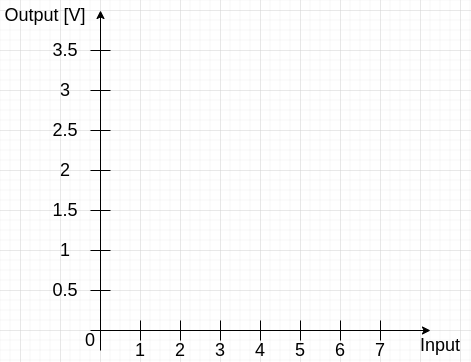
\includegraphics[width=.5\textwidth]{erreur-conversion_axes.png}
	\end{center}
}
{
	Caractéristique \textit{idéale} :
	\begin{center}
		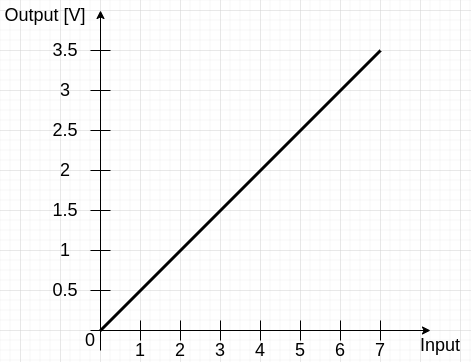
\includegraphics[width=.5\textwidth]{erreur-conversion_axes_ideal.png}
	\end{center}

	Caractéristique \textit{parfaite} en trait continu :
	\begin{center}
		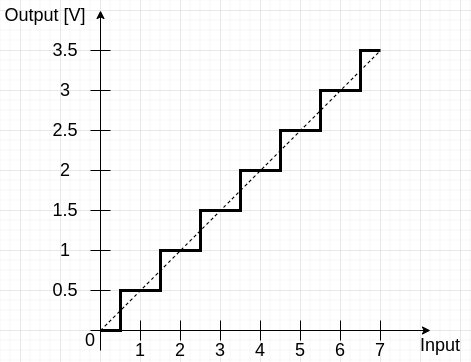
\includegraphics[width=.5\textwidth]{erreur-conversion_axes_parfait.png}
	\end{center}
}

\Question{
	Le profil de quantification est l'écart entre le signal réel et sa conversion numérique au cours du temps.
	Tracez le profil de quantification d'un convertisseur parfait pour le signal suivant.
	Considérez un converstisseur dont la résolution en tension est de 0.5~V et dont le code change à 0.75 V, 1.25 V, 1.75 V, etc.

	Commencez par tracer la sortie du convertisseur dans le même repère.

	\begin{center}
		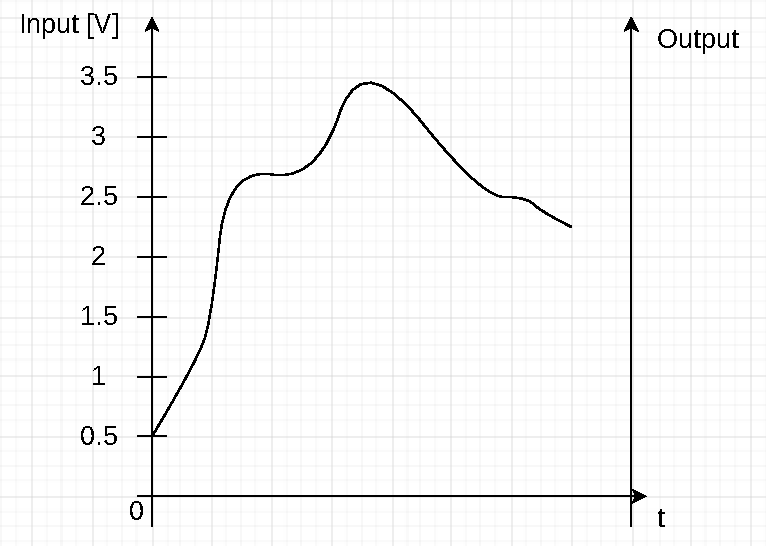
\includegraphics[]{profil-quatification.pdf}
	\end{center}

}
{
	\begin{center}
		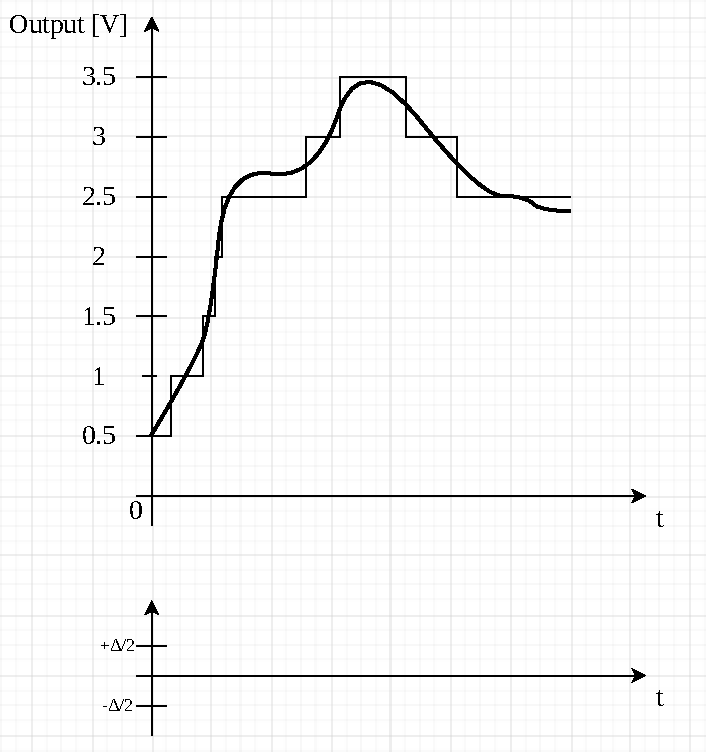
\includegraphics[width=.7\textwidth]{profil-quatification-conv-profil.pdf}
	\end{center}
}

\Question{
	En supposant une tension de référence de 8 V et un ADC sur 3 bits, donnez le code binaire correspondant à la conversion du signal ci-dessous à chaque instant d'échantillonnage (sampling pulse).
	\begin{center}
		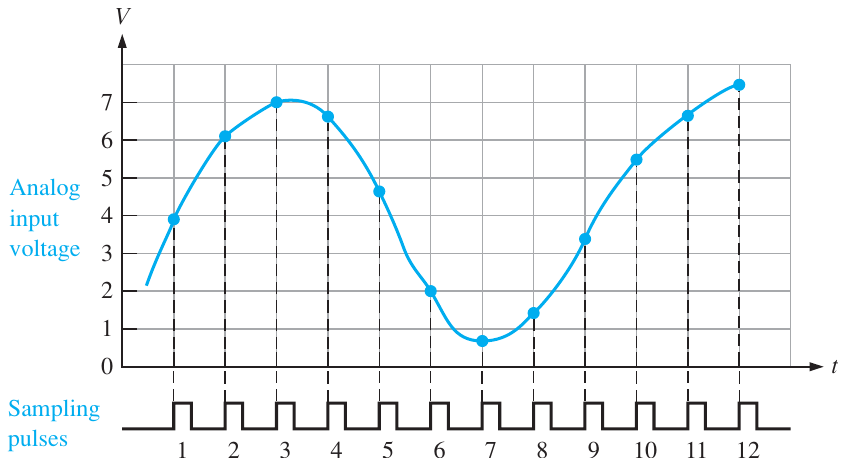
\includegraphics[width=.7\textwidth]{Floyd_fig 14-29 _ ADC sampling.png}
	\end{center}

}
{
	On obtient la séquence 100, 110, 111, 110, 100, 010, 000, 001, 011, 101, 110, 111.
}

\Question{
	Dans un DAC 4 bits en chaîne de résistances, si la résistance la plus faible est de $10k\Omega$, quelles sont les valeurs des autres résistances ?
}
{
	Les autres résistances seront une puissance de 2 de cette résistance la plus faible : $20k\Omega$, $40k\Omega$ et $80k\Omega$.
}

\Question{
	Pour le DAC représenté ci-dessous, donnez l'allure de la tension de sortie pour les différents codes binaires représentés à droite.
	\begin{center}
		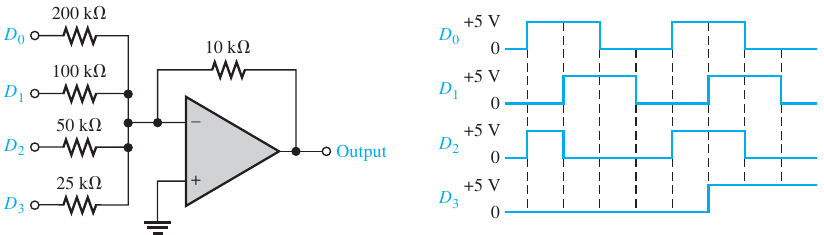
\includegraphics[width=.9\textwidth]{Floyd_fig 14-65 DAC code.png}
	\end{center}

}
{

}

\Question{
	Vous souhaitez analyser la consommation électrique de votre réseau domestique en temps réel. Pour ce faire, vous allez utiliser une pince ampèremétrique de 1000:1 (1 A devient 1 mA) reliée à un ADC (alimenté en 5 V) via une résistance de shunt de $1 \Omega$ (1 A devient 1 V).
	Sachant que votre disjoncteur principal supporte 32 A et que vous voulez mesurer jusqu'à une puissance de 1 mW, quelle devrait être la résolution de votre ADC ?

	Critiquez le résultat obtenu.
}
{
	Le réseau domestique fonctionne avec une tension sinusoïdale de 230 $V_{eff}$.
	La puissance consommée sur notre réseau domestique est donnée par $P = V \cdot I$.

	Notre disjoncteur pouvant supporter 32 A maximum, nous avons une puissance maximale sur notre réseau de $7360 W$.

	Une puissance de 1 mW correspondrait alors à un courant de 4.35 mA. Étant donné le rapport 1000:1 de la pince, ce courant correspond à $4.35\mu V$ à l'entrée de l'ADC.
	La tension \textit{full scale} de ce dernier étant de 5 V, nous avons une résolution $5 \cdot 1/2^n-1 = 4.35 \cdot 10^{-6} \Leftrightarrow  n = \log_2(\frac{5}{4.35 \cdot 10^{-6}}+1) = 20.13$. En arrondissant vers le haut, on obtient qu'il faut un ADC de 21 bits. Pour prendre en compte le bruit du signal, il vaudra sans doute mieux prendre un ADC de 24 bits.

	Cependant, notre réseau ne devrait pas s'approcher des limites de notre disjoncteur. On serait sans aucun doute à moins de 80\% du maximum si le réseau est correctement dimensionné.
	De plus, la puissance maximale actuelle du réseau, $7360 W$ correspond à une tension de $32 mV$ à l'entrée de l'ADC. En supposant une résolution de $4.35\mu V$, cette tension correspond à un code binaire $(32 mV/4.35\mu V)_{10} = (1110010111101)_2$, ce qui signifie qu'il ne faut que 13 bits pour représenter notre valeur maximale. Si nous avons effectivement sélectionné un ADC de 21 bits, les 8 bits de poids forts ne seront jamais utilisés et donc gâchés.
	On pourrait donc utiliser une pince ampèremétrique avec un rapport de transformation inférieur, une résistance de shunt plus élevée ou un amplificateur préliminaire. Cette dernière solution est sans doute la plus flexible, mais la moins bonne à cause des erreurs que l'amplificateur peut lui-même introduire dans le montage.
}

\Question{
	Vous avez en annexe un extrait de datasheet d'un ADC flash AD7829.
	\begin{enumerate}
		\item Quelle est sa résolution ?
		\item Quelles sont ses erreurs ?
		\item Si la tension de référence est de 2.5 V, quelle plage de tension est représentée par 1 LSB ?
	\end{enumerate}

}
{
	\begin{enumerate}
		\item 8 bits
		\item \begin{itemize}
			\item INL : $\pm$ 0.75 LSB
			\item DNL : $\pm$ 0.75 LSB
			\item Offset : $\pm$ 1 LSB
			\item Gain : $\pm$ 2 LSB
		\end{itemize}
		\item 1 LSB = $\frac{V_{REF}}{2^n-1} = 0.0098 V$
	\end{enumerate}
}

% \Question{

% }
% {

% }


\includepdf[pages={3,8},scale=0.9,pagecommand={\pagestyle{plain}}]{datasheet/AD7829.pdf}
\end{document}
